
%(BEGIN_QUESTION)
% Copyright 2006, Tony R. Kuphaldt, released under the Creative Commons Attribution License (v 1.0)
% This means you may do almost anything with this work of mine, so long as you give me proper credit

Calculate values for the following calibration table, for a displacer-style transmitter measuring water flow through a V-notch weir.  The displacer is cylindrical in shape, has a length of 12 inches (matching the weir's V-notch depth), and a diameter of 2 inches.  The percentage in the calibration table refers to percent of the weir's flow range, not the percentage of displacer submergence:

$$\includegraphics[width=15.5cm]{i00684x01.eps}$$

Be sure to show your work!

% No blank lines allowed between lines of an \halign structure!
% I use comments (%) instead, so that TeX doesn't choke.

$$\vbox{\offinterlineskip
\halign{\strut
\vrule \quad\hfil # \ \hfil & 
\vrule \quad\hfil # \ \hfil & 
\vrule \quad\hfil # \ \hfil & 
\vrule \quad\hfil # \ \hfil \vrule \cr
\noalign{\hrule}
%
% First row
Water flow & Percent of & Depth that displacer & Buoyant \cr
%
% Another row
rate (ft$^{3}$/s) & flow span (\%) & is submerged (in) & force (lb) \cr
%
\noalign{\hrule}
%
% Another row
  & 0 &  &  \cr
%
\noalign{\hrule}
%
% Another row
  & 10 &  &  \cr
%
\noalign{\hrule}
%
% Another row
  & 25 &  &  \cr
%
\noalign{\hrule}
%
% Another row
  & 50 &  &  \cr
%
\noalign{\hrule}
%
% Another row
  & 75 &  &  \cr
%
\noalign{\hrule}
%
% Another row
  & 90 &  &  \cr
%
\noalign{\hrule}
%
% Another row
  & 100 &  &  \cr
%
\noalign{\hrule}
} % End of \halign 
}$$ % End of \vbox


\underbar{file i00684}
%(END_QUESTION)





%(BEGIN_ANSWER)

% No blank lines allowed between lines of an \halign structure!
% I use comments (%) instead, so that TeX doesn't choke.

$$\vbox{\offinterlineskip
\halign{\strut
\vrule \quad\hfil # \ \hfil & 
\vrule \quad\hfil # \ \hfil & 
\vrule \quad\hfil # \ \hfil & 
\vrule \quad\hfil # \ \hfil \vrule \cr
\noalign{\hrule}
%
% First row
Water flow & Percent of & Depth that displacer & Buoyant \cr
%
% Another row
rate (ft$^{3}$/s) & flow span (\%) & is submerged (in) & force (lb) \cr
%
\noalign{\hrule}
%
% Another row
0 & 0 & 0 & 0 \cr
%
\noalign{\hrule}
%
% Another row
0.208 & 10 & 4.777 & 0.542 \cr
%
\noalign{\hrule}
%
% Another row
0.520 & 25 & 6.892 & 0.782 \cr
%
\noalign{\hrule}
%
% Another row
1.040 & 50 & 9.094 & 1.032 \cr
%
\noalign{\hrule}
%
% Another row
1.561 & 75 & 10.70 & 1.214 \cr
%
\noalign{\hrule}
%
% Another row
1.873 & 90 & 11.50 & 1.306 \cr
%
\noalign{\hrule}
%
% Another row
2.081 & 100 & 12 & 1.362 \cr
%
\noalign{\hrule}
} % End of \halign 
}$$ % End of \vbox

%(END_ANSWER)





%(BEGIN_NOTES)


%INDEX% Calibration: table, flow transmitter

%(END_NOTES)


